\scanpage{61}
% His upper-right number; only the lower, open oval frame survives at the clipped top edge.
\mspage{\makebox[0pt][l]{\begin{tikzpicture}[overlay,baseline=0pt]
\draw (-.22,.15) .. controls (-.24,-.22) and (.55,-.22) .. (.54,.15);
\end{tikzpicture}}18}
with $k$ a successor of $i$, it is a matter of an isolated singularity, but in the case of a general $\mathcal{V}_{i,k}^k$, one can of course find singularities of arbitrary type in the fiber (take $X_i=X_i^*$ reduced to a point !) — which diminishes the interest, in the case of stratifications that are at all general, of the general $\mathcal{V}_{i,k}^j$ as ``stones''. The $\mathcal{V}_{i,k}^{j}=\mathcal{V}_{i,k}^*$ are already more interesting, for \deleted{\unsure{these are}} it is essentially a \inserted{germ of an} open subset of $X_k^*$, hence nonsingular — which \unsure{will be expressed|is expressed} by the fact that one obtains it as a bundle over nonsingular $X_i^*$, with nonsingular fiber $\mathcal{V}_{\unsure{z|Z},Z_{i,k}}^*$ \ldots

Thus in what follows we shall systematically try to express as much as possible with the $X_i^*$ and \inserted{the} ``elementary'' $\mathcal{V}_{i,j}$, $\mathcal{V}_{i,j}^*$ ($j$ a successor of $i$), then see whether certain expressions can take a nicer form by also using \inserted{the $X_i^*$ and} the $\mathcal{V}_{\unsure{i,j|ijj}}$, $\mathcal{V}_{i,j}^*$ with $i\leq j$ \unsure{without|in} more — and only at a final stage, perhaps (\unsure{in|having} regard to the case of divisors \unsure{with|:} normal crossings) see how the $\mathcal{V}_{i,k}^j$ fit into this formalism.
% Pale lower-left foliation, another hand.
\margin{60}
